\documentclass{article}

% if you need to pass options to natbib, use, e.g.:
%     \PassOptionsToPackage{numbers, compress}{natbib}
% before loading neurips_2018

% ready for submission
% \usepackage{neurips_2018}

% to compile a preprint version, e.g., for submission to arXiv, add add the
% [preprint] option:
%     \usepackage[preprint]{neurips_2018}

% to compile a camera-ready version, add the [final] option, e.g.:
     \usepackage[final]{nips_2018}

% to avoid loading the natbib package, add option nonatbib:
%     \usepackage[nonatbib]{neurips_2018}

\usepackage[utf8]{inputenc} % allow utf-8 input
\usepackage[T1]{fontenc}    % use 8-bit T1 fonts
\usepackage{hyperref}       % hyperlinks
\usepackage{url}            % simple URL typesetting
\usepackage{booktabs}       % professional-quality tables
\usepackage{amsfonts}       % blackboard math symbols
\usepackage{nicefrac}       % compact symbols for 1/2, etc.
\usepackage{microtype}      % microtypography
\usepackage{graphicx}
\usepackage{subfig}

\usepackage{arydshln} %for dashed lines

\title{Modular Inverse Classification using Generative Models}

% The \author macro works with any number of authors. There are two commands
% used to separate the names and addresses of multiple authors: \And and \AND.
%
% Using \And between authors leaves it to LaTeX to determine where to break the
% lines. Using \AND forces a line break at that point. So, if LaTeX puts 3 of 4
% authors names on the first line, and the last on the second line, try using
% \AND instead of \And before the third author name.

\author{%
  Marius Hobbhahn \\
  Department of Computer Science\\
  University of Tübingen\\
  Tübingen, Germany \\
  \texttt{marius.hobbhahn@gmail.com} \\
  % examples of more authors
  % \And
  % Coauthor \\
  % Affiliation \\
  % Address \\
  % \texttt{email} \\
  % \AND
  % Coauthor \\
  % Affiliation \\
  % Address \\
  % \texttt{email} \\
  % \And
  % Coauthor \\
  % Affiliation \\
  % Address \\
  % \texttt{email} \\
  % \And
  % Coauthor \\
  % Affiliation \\
  % Address \\
  % \texttt{email} \\
}

\begin{document}

\maketitle


%TODO image captions in slightly different style. Like in BA
%TODO fix the tables in the appendix
\begin{abstract}
	In this paper we investigate whether temporal gradient information of generative models can be used to classify previously unseen data points. For this we show that generative models are able to reconstruct previously unseen data points. When using a modular setup, i.e. one generative network for every class we show that every generative model reconstruct the correct class best. Finally, the concept of modular inverse classification is introduced which combines the usage of gradient information to classify with the modular approach. It is tested and compared to a conventional way of classification and is able to significantly outperform it on two datasets. 
\end{abstract}

\section{Introduction}

Using temporal gradient methods has been shown to produce goal-directed behavior in the domain of planning future trajectories in partially observable environments \cite{RocketballOtte2017}.
The model has been successfully extended to not only include the prospective inference but also a retrospective inference process, i.e. inferring the unobservable contextual state that best explains its recently encountered sensorimotor experiences \cite{REPRISE2018}.
The question of this paper is whether the accomplishments of temporal gradient methods are transferable to classification tasks. 
Creating models that achieve accuracy with low amounts of training data is important because many datasets have only very few data points available. Medical trials, for example often have high cost for every added data point or in cases of rare diseases data points are just not available. \\
Using a generative model instead of a forward model is important because of the accuracy and robustness it provides. A generative model is able to create previously unseen data when the latent space is well defined. In comparison a forward model often behaves more like an upgraded lookup table and does not generalize that well. This behaviour also makes it less robust in many cases, i.e. misclassifying outliers or being easier to attack by people with malicious intent. \\
In my bachelor thesis \cite{HobbhahnBA2018} I already tested whether inverse classification is possible in general. This is an extension on my thesis where instead of using one big generative model, multiple small generative models are used in a modular fashion. The result from \cite{HobbhahnBA2018} shows that learning one big generative model for all classes leads to a very irregular latent space, likely because it is too complex of a task for a model of this size. S. Otte showed in \cite{2019_icann_dynamics} that in such situations the problem can be solved by using modular approaches by distributing and thereby reducing the complexity per model. Z. Lipton and S. Tripathi investigate the latent vectors generated from the inverse mapping of images with GANs in \cite{LatentVectors2017}. They also show that previously unseen images converge to reasonable representations in latent space, however they do neither investigate how good classification works with this technique nor do they test a modular approach. 
\par

This work investigates three main questions: a) Is Inverse Classification able to construct previously unseen patterns, can it reconstruct the pattern by only using temporal gradient information? b) Is modular Inverse Classification able to classify previously unseen data correctly, i.e. does the reproduced pattern have the smallest error to the true target vs. other targets? c) Is Modular Inverse Classification, i.e. the combination of small modular generative networks, able to outperform a standard forward approach trained on similar data? This is the main question of the report and therefore tested and analyzed in multiple subexperiments. Those consist of testing different datasets as basis for the generative models, adding noise to the input and output features, analyzing the functionality of gradient methods and comparing it to conventional forward classification.

\section{Inverse Classification using Generative Models}
\label{sec:ICGM}

The main innovation of this paper is inverse classification using generative models. This means to first train a generative model to learn to generate sequences. In the second step this model is then used to inversely classify data by generating sequences with an input vector. The sequences are then compared to the target and the input vector is iteratively adapted through gradient based methods. A more detailed explanation of the two step process can be found in the following two sections.

\subsection{Sequence Generation}

A recurrent neural network with LSTMs is trained to generate sequences from class inputs. The classes are represented as one-hot vectors, i.e. vectors where one entry is one and all others are zero. The model gets the class information only in the very first timestep, being fed zero values for the rest. The model generates one part of the sequence at every point in time, not a one shot at the end. The sequences generated in this paper are two dimensional and represent the coordinates of a handwritten character trajectory. In principal every generative network could be used to inversely classify but since sequential data are being used, a recurrent model seemed appropriate. A graphical depiction of the process can be found in Figure \ref{fig:generative_model}.

\begin{figure}[!htb]
	\centering
	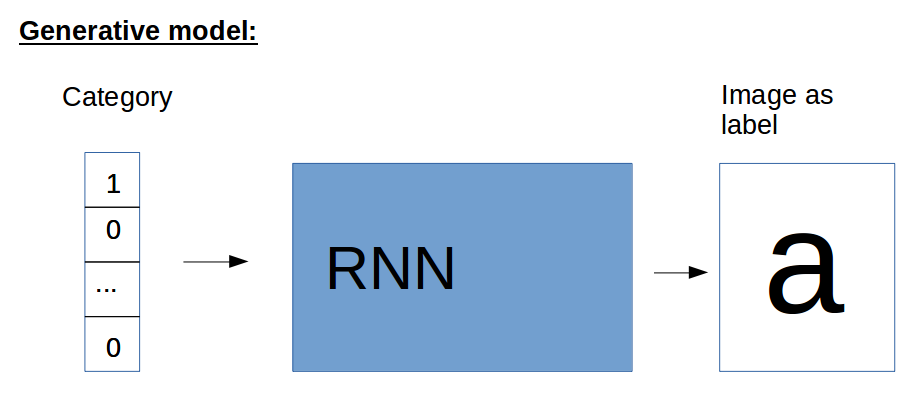
\includegraphics[width=\textwidth]{images/generative_model.png}
	\caption{Depiction of the sequence generation.}
	\label{fig:generative_model}
\end{figure}

\subsection{Inverse Classification}

The fully trained generative model is now used for inverse classification. Importantly, during the entire classification process the network weights are not changed. The success of the classification relies only on the concepts learned during the generative training. To classify a given target sequence, a character is generated. Since there is no prior information which character the target might be, the first generation is always performed from a uniformly distributed input vector. The resulting sequence is then compared to the sequence representing the target and an error is calculated. The gradient of the first layer of the network with respect to that error is then calculated and the uniformly distributed vector can be adapted proportional to the gradient. This process is done multiple times either until the input converges towards a static vector or the classification process is stopped after a given amount of steps. In the optimal case the input converges towards the one-hot vector representing the class of the target. Mathematically speaking, the inverse classification can be thought of as the inverse function to the generation. This implies that $f^{-1}(f(x)) = x$ if the inverse classification process works optimal, where $f(x), f^{-1}(x)$ denote the generative network and inverse classification respectively. A graphical interpretation of the process can be found in Figure \ref{fig:inverse_classification}. 

\begin{figure}[!htb]
	\centering
	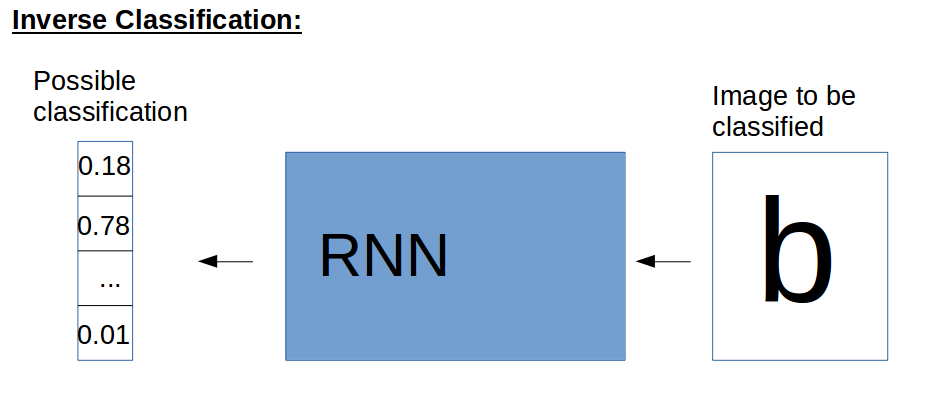
\includegraphics[width=\textwidth]{images/inverse_classification.png}
	\caption{Depiction of the inverse classification. The generative network (in this case a RNN) reconstructs the character by using the temporal gradient information until it converges to a vector. A possible classification vector is represented in the left}
	\label{fig:inverse_classification}
\end{figure}

\subsection{Extension to Modular Approach}
\label{subsec:extension_to_MC}

To modularize Inverse Classification a separate generative network is trained for every data class, i.e. for every character. To classify a previously unseen data point every network inversely classifies the data point resulting in a reconstruction. Given that most networks are not able to reconstruct a sequence that is very different from the one to be classified their reconstruction either collapses like the `z' in Figure \ref{fig:modular_inverse_classification} or it is an adapted version of the character that was learned by the model like the `a' in the same figure. Every reconstruction is then compared to the character to be classified. The comparison was done by a mean squared error distance measure. A Dynamic Time Warping (DTW) Distance could also have been used and is a suggestion for future research. 

\begin{figure}[!htb]
	\centering
	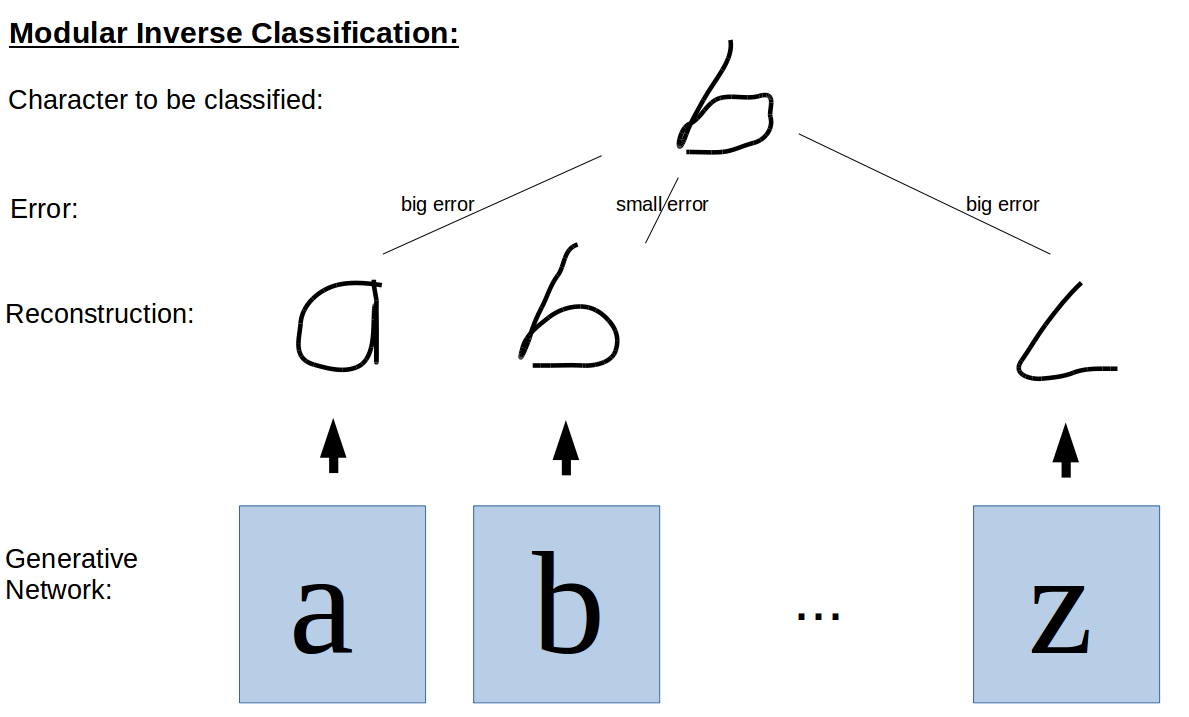
\includegraphics[width=\textwidth]{images/modular_inverse_classification.png}
	\caption{Depiction of the modular inverse classification. In the top row is a depiction of the character we want to classify. Every individual generative network in the bottom row tries to reconstruct this character by inverse classification. The resulting reconstructions, shown in the third row, is now compared to the to be classified character. The reconstruction with the lowest error is chosen as the winner.}
	\label{fig:modular_inverse_classification}
\end{figure}

\section{Experiments}

In this section three experiments are introduced. The first two are necessary conditions for modular inverse classification (MIC) and the results are therefore discussed already with the introduction of the experiments. The main experiments is split into four subexperiments that are detailed in Subsection \ref{subsec:modular}.


\subsection{Data}
\label{subsec:data}

\subsubsection{UCI Character Sequences}

The data are handwritten digits taken from the UCI Machine Learning Repository Character Trajectories Data Set from 2008 \cite{uci2013}. 
It contains only characters that can be written in a single stroke, leading to 20 different classes with 2858 example characters in total. The six remaining letters of the alphabet are left out since they cannot be written within a single stroke. \\
Originally the digits are saved with x- and y- delta values, i.e. the difference between two following points and a z-value representing the pin pressure used during the process of writing. For this work the cumulative sum of the deltas are taken to get the absolute coordinates for the training and the values for pin pressure are removed. A network trained on deltas instead of coordinates performed worse and the pin pressure did not add predictive value.
The data are padded with the last coordinate such that all have the same length but no information is added or removed. 
Additionally, the individual characters are standardized globally with mean 0 and standard deviation 1. Standardization leads to slightly better predictions. 
For every experiment the data are split into 80\% training and 20\% test data. The test data are not used for validation during training but only after the training is finished.
Lastly, it should be noted that the characters are often hard to distinguish even for humans. In figure	\ref{fig:hard_characters}
a cherry-picked 'u' is depicted on the left and a cherry-picked 'w' on the right. This fact makes the classification more complicated. 

\begin{figure}[!htb]
	\centering
	\begin{tabular}{cc}
		\subfloat[]{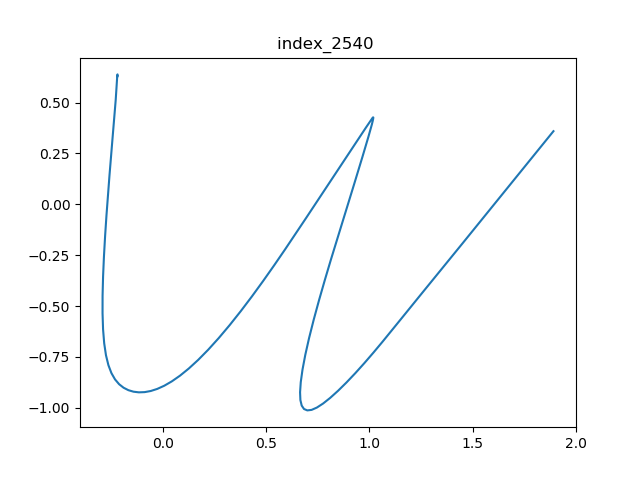
\includegraphics[width=5cm]{images/char_u_index_2540.png}} 
		& \subfloat[]{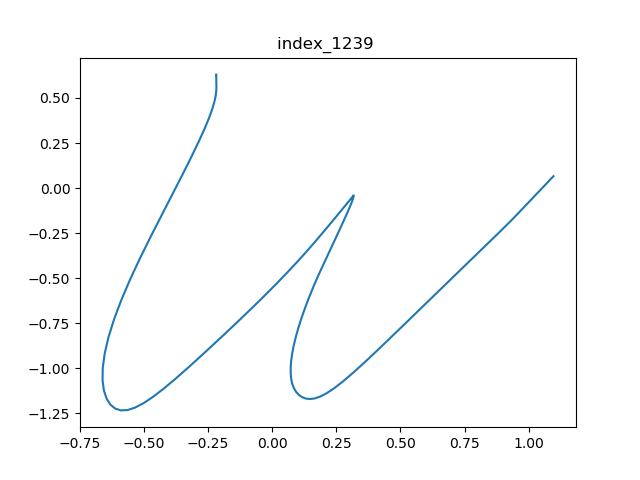
\includegraphics[width=5cm]{images/char_w_index_1239.png}}
	\end{tabular}
	\caption{On the left the character 'u' and on the right the character 'w' is depicted as they are found in the data set. Since they are rather similar in look the network might have additional difficulties separating them accordingly.}
	\label{fig:hard_characters}
\end{figure}

\subsubsection{(sequential) MNIST}

MNIST is a large database of handwritten digits. Every image is represented as a 28 by 28 pixel grey scale image. In total there are 60000 training and 10000 test images. In the experiments of this paper, the pixel values are normalized. In other applications such as image classification every image is fed into the network as a whole. In this application we use (sequential) MNIST sometimes also referred to as pixel MNIST which means that every image is read in as a sequence of 28 pixel rows of size 28. 


\subsection{Setup of the Networks}
\label{subsec:setup}

Every generative network is a LSTM with 10 cells for the character sequences and 20 cells for MNIST. It is trained on four different sequences that represent different types of a particular character. How these types are chosen is shown in the Modular Approach Subsection \ref{subsec:modular}. Every network is trained until the types have been learned perfectly, i.e. the mean squared error is close to zero. This is achieved by training for 40000 episodes per network for the character sequences and 20000 episodes per network for MNIST. As an optimizer Adam \cite{AdamKingmaB14} was used with learning rate 0.01 and otherwise standard parametrization. All inverse classification experiments were implemented in python3 using Pytorch \cite{Pytorch}. The comparison to forward classification was implemented using keras \cite{chollet2015keras}. All code can be found online at 
\url{https://github.com/mariushobbhahn/Modular-Inverse-Classification}.

\subsection{Reconstruction of previously unseen Patterns}
\label{subsec:reconstruction}

A necessary precondition for inverse classification in general is that the generative network is able to reconstruct previously unseen patterns. This means that it fits the character sequence by adapting its states through the temporal gradient information. The tests for the reconstruction are done in a qualitative manner and shown in Figure \ref{fig:unseen_fit_MNIST} and \ref{fig:unseen_fit_chars} for the MNIST and the character sequences respectively. In the top row of the figure the data points on which the network was trained are shown. It is important to stress that those points are the only representatives of zeros the network has ever seen. In the second row the test targets are shown. The network is given such a sequence and is tasked with reconstructing such an image only through the gradient information. In the bottom row the reconstruction of the network with the respective gradients is given. There are two findings from the two figures. First, the reconstructions all significantly differ from the original four training points, meaning that the network can construct previously unseen patterns. Evidence for this can be found in both figures, however, in the character sequences case it is very prominent. The line of the character `a' in target 2 shows a sharp bend which none of the types the network is trained on shows. Still the network is able to account for that sharp bend in prediction 2. Second, the reconstruction is done in a way that is a combination of the previously seen images with adaptions. Prediction 2 in the MNIST figure \ref{fig:unseen_fit_MNIST}, for example, is a combination of 0.22 type 1 and 0.78 type 2. However, it very likely is a non-trivial combination, given that a human might rather choose type 0 to reconstruct target 2. An extreme case for the combination aspect is shown in prediction 3 of the character sequences where the network reconstructs target 3 entirely from type 0 if the gradient information is to be believed. 

\begin{figure}[!htb]
	\centering
	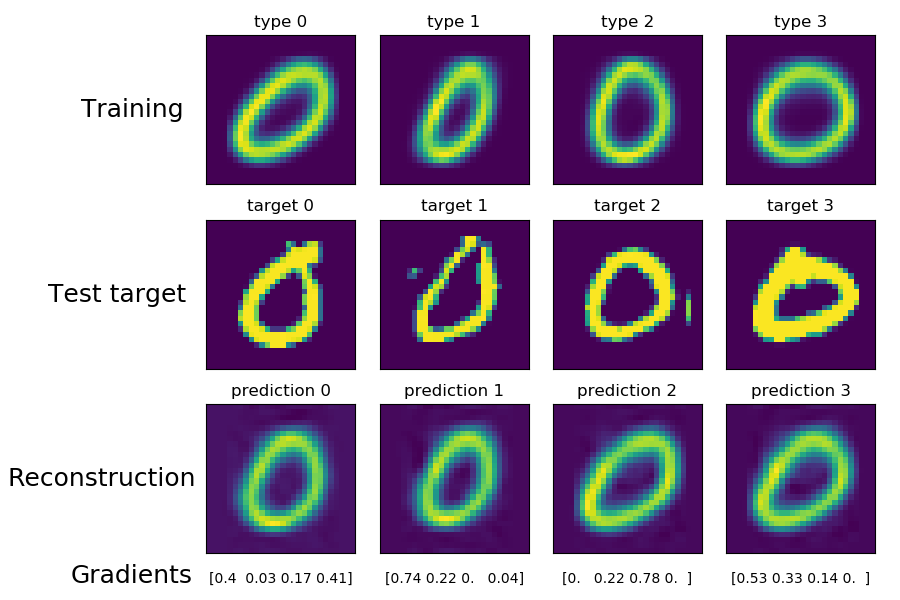
\includegraphics[width=\textwidth]{images/MNIST_IC.png}
	\caption{Reconstruction of previously unseen (sequential) MNIST images. In the upper row are the four samples the networks has been trained on. In the second row are the test targets the network is supposed to reconstruct and in the third row are said reconstructions with the respective final gradients. From this comparison it is clear that the network is able to reconstruct images that it has never seen during training through gradient information.}
	\label{fig:unseen_fit_MNIST}
\end{figure}

\begin{figure}[!htb]
	\centering
	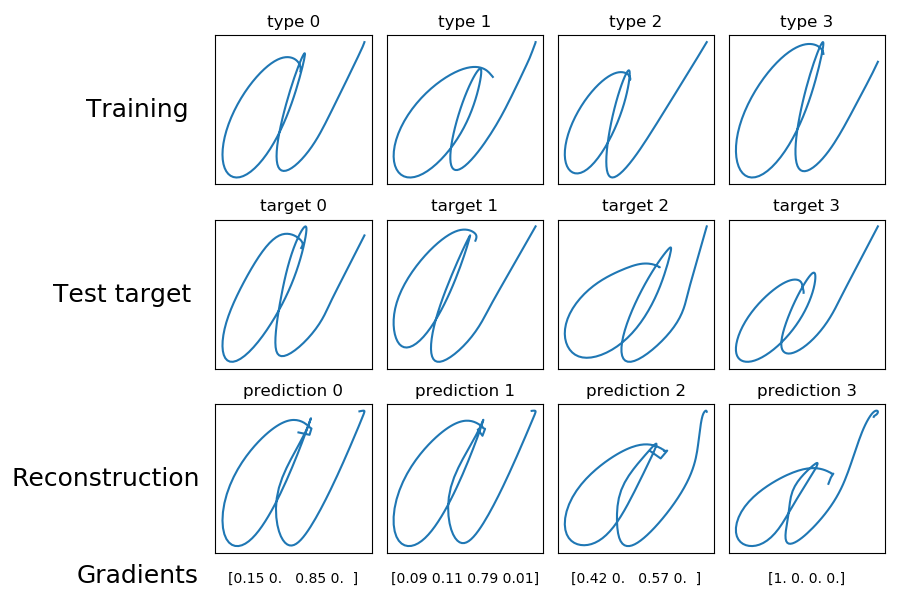
\includegraphics[width=\textwidth]{images/chars_IC.png}
	\caption{Reconstruction of previously unseen handwritten character sequences. In the upper row are the four samples the networks has been trained on. In the second row are the test targets the network is supposed to reconstruct and in the third row are said reconstructions with the respective final gradients. From this comparison it is clear that the network is able to reconstruct sequences that it has never seen during training through gradient information.}
	\label{fig:unseen_fit_chars}
\end{figure}


\subsection{Classification of previously unseen Data}
\label{subsec:classification}

To test whether modular Inverse Classification is a promising approach every generative model is tested to reconstruct every character or every number. This is done by taking 20 previously unseen sequences and inversely classifying. A heat map of the reconstruction loss, i.e. average mean squared error between target and reconstruction is created. In the optimal case there are dark entries on the diagonal and light entries everywhere else. This means that every generative network exactly classifies the character/digit it is supposed to classify and no other. However, given the similarities between some characters like `u' and `w' in handwritten digits or the similarities between `8' and `9', for example, their difference should also be smaller. It is important to point out that there is an inherent trade-off between the flexibility of the generative models and its accuracy. The higher the flexibility of the generative model the more likely it is to not only reproduce the correct class but also fit samples of a incorrect class, thereby increasing the misclassification rates. The best performing model for the clustered subsets of both the MNIST and the character sequences datasets have been tested according to the just described procedures. The results are shown in Figure \ref{fig:heatmaps}. In the upper row the results for the character sequences on the training data and the test data can be seen on the left and right respectively. In the lower row the results for MNIST are displayed, also showing the reconstructions on the trainingsset on the left and on a test set on the right. In all cases the darkest entries per row and column lie on the diagonal. That means on average our model reconstructs the the character it is supposed to reconstruct best. The reconstruction of previously unseen data, which is depicted in the right column of the figure, is slightly worse than those of the training data, but still sufficiently good given the darkness of the diagonal entries. 

\begin{figure}[!htb]
	\centering
	\begin{tabular}{cc}
		\subfloat[]{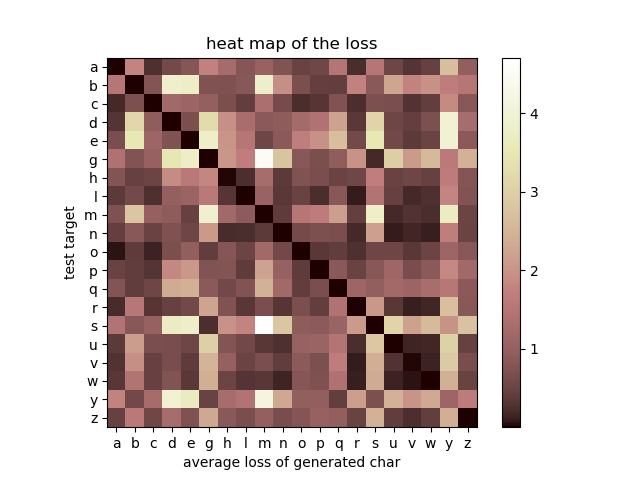
\includegraphics[width=8cm]{images/cross_loss_dtw_in_01_out_00002.png}} 
		& \subfloat[]{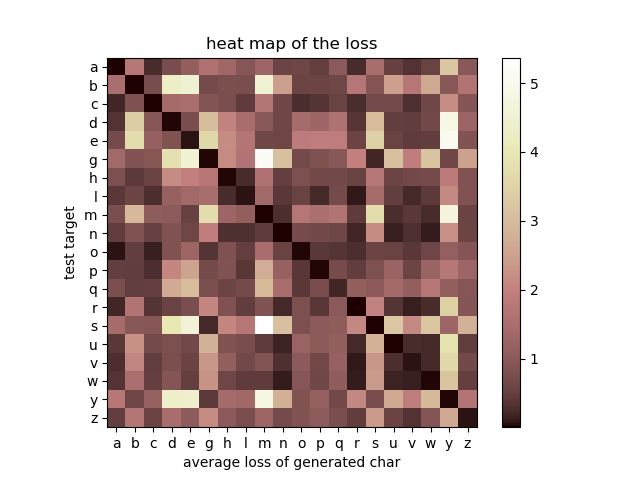
\includegraphics[width=8cm]{images/cross_loss_dtw_in_01_out_00002_test.png}} \\
		\subfloat[]{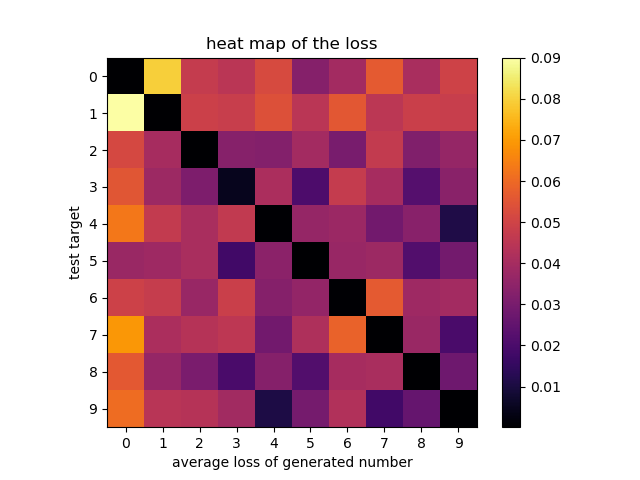
\includegraphics[width=8cm]{images/loss_cross_MNIST_in_02_out_01_train.png}} 
		& \subfloat[]{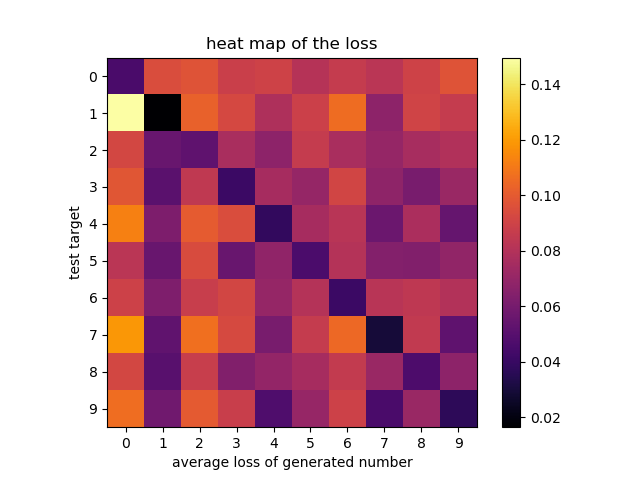
\includegraphics[width=8cm]{images/loss_cross_MNIST_in_02_out_01_test.png}} 
	\end{tabular}
	\caption{Heat map of the loss for character sequences and MNIST dataset for train and test data. Each heat map is constructed by taking the average loss of the reconstruction of a data point and the true data point for all models and all data points. a) character sequences train data b) character sequences test data c) MNIST train data d) MNIST test data}
	\label{fig:heatmaps}	
\end{figure}	

\subsection{Modular Approach}
\label{subsec:modular}

As already motivated in the introduction a generative network trained on all input sequences is not able to provide inverse classifications that outperform the conventional forward approach but only ones that are similarly good in some circumstances. This result is likely the case because the latent space of that size is not very smooth when trained with LSTMs. To solve this problem a modularity is introduced like described in Subsection \ref{subsec:extension_to_MC}. To test whether the modularity works multiple experiments are described in the following.

\subsubsection{Clustered versus Random Training Samples}

To train the modular Inverse Classification (MIC) networks training samples are needed. Since a subset of the entire dataset is chosen for both the MNIST and the character sequences we need to specify a mechanism for that choice. Here we use two mechanisms. First, a clustered sampling that is chosen by K-means clustering with the DTW-distance for the character sequences and Euclidean distance for the MNIST dataset as metrics. This is supposed to be a best case test, i.e. how good is MIC if we have samples that are good representatives of the underlying distributions. Second, we use random sampling, i.e. choose four random samples per class (seed is 42). This is supposed to be an average case test, i.e. how good is MIC if we have very few samples that are average representatives of the dataset. The experiment is a comparison of the overall and per class accuracies of the models trained on clustered and random datasets respectively. 

\subsubsection{Addition of Noise on input and output}

There are two complications with modular Inverse Classification (MIC) that can be solved through the addition of noise. First, the latent space is not very smooth because the network only trains on one-hot vectors. This can be helped with adding noise on the input, i.e. Gaussian noise with mean 0 and standard deviation $\sigma$. Additionally the new input vector is clipped at 0 and 1 such that the network does not see values smaller than 0 or bigger than 1. This primarily serves the purpose of smoothing the latent space such that the small steps along the gradient that MIC uses can be used to converge and have no abrupt breaks. Second, the number of samples is very restricted in our settings. by adding noise on the output data we hope to simulate variations in those data points and thereby enhancing the performance of the model. In the experiments multiple values for the noise parameters are added to the data where only the standard deviation of the Gaussian noise $\sigma$ is changed. The addition of input noise is similar for both datasets, given that both use a one-hot encoding for their sequences generation. The noise added on the output data is different because the addition of noise on a sequence of coordinates is way more destructive than on image pixels. In addition to the overall accuracy the per class accuracy is also reported. To test whether the noise had a positive influence a generalized linear model (GLM) with binomial model family and logit link function was chosen. Given the problems with p-Values, especially in settings with few data points the coefficients for the different noise levels will be treated as a trend and not a proof.

\subsubsection{Distinction between Modular Approach with and without Inverse classification}

It could be argued that the positive results of the modular Inverse Classification (MIC) stem only from the modularity of the network and not from the gradient information. To test the influence that the inverse part of MIC has we compare the results of the MIC after 0 and 50 iterations on previously unseen data. MIC with 50 iterations is the usual setup that was used throughout this work and is therefore representative for the approach. If there is a difference between the 0 iterations and 50 iterations case that means the gradient information has an influence on the classification. This difference is determined along two metric. The first metric is accuracy, as is fitting for a classification task. The second is the mean squared error (MSE). This metric is used because a MIC model with 50 iterations that has the same accuracy as a MIC model with 0 iterations can still fit the correctly classified data better and therefore be advantageous compared to not using the gradient information. The comparison is conducted for both datasets and both, the random and the clustered subset respectively along these two metrics. 

\subsubsection{Comparison to Forward Classification}

To establish the feasibility of the modular Inverse Classification (MIC) we compare it to the conventional forward classification approach. That is to train a network of similar size on the respective training dataset and testing its accuracy on previously unseen data. To make a fair comparison the network has the same amount of LSTM cells as the sum of all small networks in the MIC case. Note, that the same amount of cells does not imply same amount of parameters. Ten networks of 20 cells each have significantly less parameters in total than a network with 200 LSTM cells because the cross connections are not accounted for. For both, the MNIST and the character sequence dataset an individual network is trained and tested on previously unseen data. This procedure is done for the entirety of the dataset and both of the two subsets, i.e. clustered and random datapoints. 

\section{Results for Modular Inverse Classification}
\label{sec:results}

The necessary preconditions for modular inverse classification (MIC) to work were fulfilled in the previous sections. From a theoretical standpoint MIC should be able to classify previously unseen data correctly. The empirical evaluations of the main experiments is presented in the following. 

\subsection{Clustered vs Random Training Samples}
\label{subsec:clustered_vs_random_results}

The accuracies of the models without the addition of noise to input or output can be found in Table \ref{table:clustered_vs_random_results}. The MNIST models achieve an accuracy of 0.83 for clustered and 0.562 for random. In the case of the character dataset we have an accuracy of 0.88 for clustered and 0.72 for random. So in both cases, as expected, clustered dataset performs better than the one based on random samples.

\begin{table}[!htb]
	\centering
	\caption{Accuracies of models without the addition of any noise to the input or output. In both the MNIST and characters dataset the clustered version achieves better results than the random one.}
	\begin{tabular}{l | cc}
		\toprule
		Dataset & Random & Clustered \\
		\midrule
		MNIST & 0.562 & 0.83\\
		Characters & 0.72 & 0.88\\
		\bottomrule
	\end{tabular}
	\label{table:clustered_vs_random_results}
\end{table}


\subsection{Addition of Noise to input and output}

%just show for MNIST clustered and refer to other datasets in appendix
For purposes of readability a full analysis of the results w.r.t. the noise experiments is only conducted for the MNIST clustered dataset. For the three other datasets the main results will be reported and put into context here. The result tables can be found in the appendix in Subsection \ref{subsec:results_noise_appendix} while the other GLMs are in Subsection \ref{subsec:GLMs}. 
\par
In Table \ref{table:MNIST_clustered_results} the results for the noise experiments of the MNIST clustered dataset are depicted. There are two main observations: a) The MIC performs with different accuracy when classifying different numbers, i.e. classifying a `1' has on average a significantly higher accuracy than classifying an `8'. This is important information because it can influence future decisions w.r.t. data collection. b) adding noise seems to be generally positive. To test how positive exactly, we conduct the results from the GLM shown in Table \ref{table:MNIST_clustered_GLM}. The coefficients for the input noise are positive, implying a positive influence w.r.t. accuracy. The coefficient for small output noise is positive but small and for bigger output noise is around zero implying that some output noise can have marginal positive effects. The p-values are all non-significant, such that the just given analysis should be seen as a tendency rather than a clear effect. Both of the two just described effects are confirmed in all other three noise experiments reported in the Appendix.


\begin{table}[!htb]
	\centering
	\caption{Results for the addition of noise experiment for the MNIST clustered dataset. On the left the addition of noise on in- and output is shown. On the right the overall and individual accuracy for all numbers is given. The model with input noise with std. of 0.2 and output noise of 0.1 has the highest overall accuracy.}
	\begin{tabular}{rr||r|rrrrrrrrrr}
		\toprule
		noise in &  noise out &  overall &      0 &      1 &      2 &      3 &      4 &      5 &      6 &      7 &      8 &      9 \\
		\midrule
		0.0 &       0.00 &    0.830 &  0.918 &  0.992 &  0.759 &  0.748 &  0.773 &  0.862 &  0.908 &  0.778 &  0.764 &  0.798 \\
		0.1 &       0.00 &    0.861 &  0.929 &  1.000 &  0.819 &  0.841 &  0.691 &  0.897 &  0.943 &  0.838 &  0.742 &  0.915 \\
		0.2 &       0.00 &    0.858 &  0.918 &  0.984 &  0.828 &  0.860 &  0.755 &  0.920 &  0.954 &  0.808 &  0.730 &  0.819 \\
		0.0 &       0.10 &    0.858 &  0.941 &  0.992 &  0.767 &  0.710 &  0.836 &  0.885 &  0.920 &  0.848 &  0.798 &  0.894 \\
		0.0 &       0.25 &    0.813 &  0.941 &  0.984 &  0.741 &  0.813 &  0.791 &  0.782 &  0.920 &  0.899 &  0.708 &  0.521 \\
		0.1 &       0.10 &    0.870 &  0.918 &  0.984 &  0.836 &  0.841 &  0.836 &  0.874 &  0.954 &  0.848 &  0.730 &  0.862 \\
		0.1 &       0.25 &    0.862 &  0.918 &  0.992 &  0.828 &  0.850 &  0.636 &  0.897 &  0.954 &  0.859 &  0.764 &  0.936 \\
		0.2 &       0.10 &    \textbf{0.873} &  0.918 &  1.000 &  0.853 &  0.841 &  0.745 &  0.874 &  0.954 &  0.848 &  0.798 &  0.894 \\
		0.2 &       0.25 &    0.868 &  0.929 &  1.000 &  0.836 &  0.785 &  0.827 &  0.851 &  0.943 &  0.869 &  0.798 &  0.830 \\
		\bottomrule
	\end{tabular}
	\label{table:MNIST_clustered_results}
\end{table}


\begin{table}[!htb]
	\centering
	\caption{GLM for the MNIST clustered noise experiments. The coefficients for the input noise are positive, indicating a positive effect. Output noise seems beneficial when only a small amount is added.}
	\begin{tabular}{lclc}
		\toprule
		\textbf{Dep. Variable:} &     Accuracy     & \textbf{  No. Observations:  } &        9    \\
		\textbf{Model:}         &       GLM        & \textbf{  Df Residuals:      } &        4    \\
		\textbf{Model Family:}  &     Binomial     & \textbf{  Df Model:          } &        4    \\
		\textbf{Link Function:} &      logit       & \textbf{  Scale:             } &    1.0000   \\
		\textbf{Method:}        &       IRLS       & \textbf{  Log-Likelihood:    } &   -2.6237   \\
		\textbf{Date:}          & Sun, 21 Jul 2019 & \textbf{  Deviance:          } & 0.0034124   \\
		\textbf{Time:}          &     00:05:01     & \textbf{  Pearson chi2:      } &  0.00341    \\
		\bottomrule
	\end{tabular}
	\begin{tabular}{lcccccc}
		& \textbf{coef} & \textbf{std err} & \textbf{z} & \textbf{P$>$$|$z$|$} & \textbf{[0.025} & \textbf{0.975]}  \\
		\midrule
		\textbf{Intercept} &       1.5711  &        2.031     &     0.774  &         0.439        &       -2.410    &        5.552     \\
		\textbf{in\_01}    &       0.2401  &        2.291     &     0.105  &         0.917        &       -4.251    &        4.731     \\
		\textbf{in\_02}    &       0.2572  &        2.299     &     0.112  &         0.911        &       -4.249    &        4.763     \\
		\textbf{out\_01}   &       0.1430  &        2.347     &     0.061  &         0.951        &       -4.458    &        4.744     \\
		\textbf{out\_025}  &      -0.0156  &        2.281     &    -0.007  &         0.995        &       -4.485    &        4.454     \\
		\bottomrule
	\end{tabular}
	\label{table:MNIST_clustered_GLM}
\end{table}

\subsubsection{Distinction between Modular Approach with 0 and 50 iterations}

The results of the comparison between MIC with 0 and with 50 iterations can be found in Table \ref{table:modular_vs_MIC}. For all four datasets MIC is compared with 0 and 50 iterations of gradient updates measured by accuracy and MSE as metrics. In all cases the results for the base model and for the model which yields the best result after 50 iterations in the respective category are shown. The later is denoted as the `best' accuracy and MSE. Since the result after 50 iterations does not mean that the model after 0 iterations is also better than the base models the entries for the `best' category for 0 iterations can sometimes be worse than the accuracy for the base model. In all cases the model with 50 iterations of gradient updates performs better than the model with 0 iterations. This is strong evidence for the usefulness of iterative gradient methods and inverse classification as a concept. 

\begin{table}[!htb]
	\centering
	\caption{Results for the comparison of MIC with 0 and 50 iterations. For all four datasets MIC is compared with 0 and 50 iterations of gradient updates. For all datasets the results for the base model and for the model with overall best accuracy for 50 iterations is shown. The values for the accuracy best column for 0 iterations are chosen from the model with the highest accuracy from 50 iterations. In all cases doing inverse classification for 50 iterations yields significantly better results than with 0 iterations.}
	\begin{tabular}{l | cccc}
		\toprule
		Dataset (\#iterations) & accuracy & accuracy best & MSE & MSE best \\ 
		\midrule
		clustered MNIST (0) & 0.705 & 0.689 & 0.059 & 0.056 \\
		clustered MNIST (50)& 0.83 & 0.873 & 0.041 & 0.039 \\
		\hdashline
		random MNIST (0) & 0.449 & 0.447 & 0.099 & 0.088\\
		random MNIST (50) & 0.562 & 0.643 & 0.076 & 0.041\\
		\hdashline
		clustered characters (0) & 0.715 & 0.768 & 0.445 & 0.226\\
		clustered characters (50) & 0.880 & 0.91 & 0.257 & 0.099\\
		\hdashline
		random characters (0) & 0.68 & 0.715 & 0.339 & 0.349\\
		random characters (50) & 0.720 & 0.818 & 0.254 & 0.196\\
		\bottomrule
	\end{tabular}
	\label{table:modular_vs_MIC}
\end{table}

\subsubsection{Comparison to Forward Classification}

The results of the conventional classification methods are displayed in Table \ref{table:forward_comparison}. For both datasets the full dataset receives the highest and a close to perfect accuracy with 0.99 and 0.973 respectively. In the restricted datasets with only four representatives per class accuracies drop significantly in both cases with 0.633 and 0.504 for MNIST and 0.613 and 0.687 for the character sequences for the clustered and random data choice mechanism respectively. In the case of the character sequences the network trained on clustered data is outperformed by the one trained on randomly chosen data. This is unexpected. One could argue that K-Means clustering returns data points that are very different from each other and this maybe influences the forward classification because most points are somewhere between the cluster centers. However, that same argument would also apply to the forward classification of the clustered MNIST dataset and both cases of inverse classification. Given that this is not the case the reason for this result remains unclear. 

\begin{table}[!htb]
	\centering
	\caption{Results for the conventional forward models. The models have been trained on the random and clustered subsets for MNIST and character sequences respectively and additionally for the entirety of the dataset. The model trained on all data outperforms the others in both cases. The model trained on the clustered samples is better for MNIST but not for the character sequences.}
	\begin{tabular}{l|ccc}
		\toprule
		Dataset &  Clustered & Random & Full \\
		\midrule
		(sequential) MNIST & 0.633 & 0.504 & 0.99 \\
		Character sequences & 0.613 & 0.687 & 0.973 \\
		\bottomrule
	\end{tabular}
	\label{table:forward_comparison}
\end{table}

\section{Conclusion}

In this paper we could show that using gradient information of a generative model to iteratively update the current best approximation of a previously unseen data point can be used for classification tasks \ref{subsec:reconstruction}. Furthermore we showed that the generative model primarily reconstructs and therefore classifies the classes it is supposed to reconstruct and not any other \ref{subsec:classification}. Lastly, it was shown that if applied in a modular fashion the technique is able to outperform conventional forward methods of classification \ref{sec:results}.
A final comparison of the most important results is shown in Table \ref{table:final_comparison}. For both datasets (MNIST/characters) and subsets (clustered/random) the accuracy of the MIC without addition of noise (base), best performing with addition of noise (best) and conventional forward classification model (forward) are compared. In all cases both MIC models outperform the forward model and are even improved through the addition of noise. The difference between the performances is not marginal but very significant, i.e. in the case of the clustered MNIST data the MIC model has an accuracy of 0.873 vs 0.633 of the forward model. This difference is even bigger for the character sequences. In the case where random samples were chosen, the difference is not as big but still substantial with 0.643 vs 0.504 and 0.818 vs 0.687. However, none of the MIC models achieve the same accuracy as a forward model trained on the entirety of the dataset. This would have been unexpected given that this is a difference of 40 vs 60000 training samples for MNIST and 80 vs 2200 trainings samples for the character sequences. In light of this massive difference in training set size the accuracies achieved by the MIC are still good for many applications. 

\begin{table}[!htb]
	\centering
	\caption{Comparison of all results. For both datasets the results for MIC without noise (base) with noise (best) and a conventional forward classification model (forward) are compared. In all cases the MIC outperforms the forward model and is improved by the addition of noise to in and output. MIC is not able to beat a forward model trained on the entirety of the dataset.}
	\begin{tabular}{l|cc}
		\toprule
		Dataset &  MNIST & Character sequences \\
		\midrule
		clustered (MIC base) & 0.83 & 0.88 \\
		clustered (MIC best) & \textbf{0.873} & \textbf{0.91} \\
		clustered (forward) & 0.633 & 0.504 \\
		\hdashline
		random (MIC base) & 0.562 & 0.72 \\
		random (MIC best) & \textbf{0.643} & \textbf{0.818} \\
		random (forward) & 0.504 & 0.687 \\
		\hdashline 
		full dataset & 0.99 & 0.973 \\
		\bottomrule
	\end{tabular}
	\label{table:final_comparison}
\end{table}


\subsection{Limitations}

Even though the technique of MIC has advantages, which are discussed in the previous parts of the paper, there are two limitations that are layed out in the following. 
%the more data, the worse on comparison (because only one representation per class) -> use GANs for better latent space
First, and most importantly, more training data does not necessarily mean a higher accuracy for MIC. The generative model is likely to converge to one representation of a class that is independent of the number of training samples it has, thereby limiting the effect of the gradient based method. This can be circumvented by training each generative model with types, i.e. giving each label a unique one-hot encoding. However, this gets very inconvenient for large datasets, especially when the number of training points is not static but gets updated over time. On the flip side, when a new training point is added only one module needs to be retrained instead of the entire forward classification model. 

%training time (parts of which are parallelizable)
Second, the time to classify a test data point is longer than in conventional methods. In the forward case the classification of a test data points needs one forward pass through the model. In the case of MIC the test point is inversely classified in every single network. This inverse classification, or reconstruction, is in itself an optimization process and therefore more expensive. However, if the hardware is available and the implementation correct, the inverse classification process for every module can be parallelized, since all modules are independent of each other.  


\subsection{Future Outlook}

In the following two ideas for future research are layed out. 
%use gans for generative model
Even though LSTMs are sufficiently good as generative models, GANs are the current state of the art and might therefore yield better results for MIC. It might even be possible not to use a modular but a holistic approach, given that GANs yield more smooth latent spaces than other generative models.

%let the model choose the types ala reprise
Another possible extension is to move higher on the abstraction hierarchy by letting the generative model infer the types of the input data instead of giving them as input. An idea similar to this has already been show to work and improve gradient based methods in \cite{REPRISE2018}. 


\bibliographystyle{alpha}
\bibliography{bibliography}

\section*{Appendix}

\subsection{Noise on input and output - Appendix}
\label{subsec:results_noise_appendix}
%MNIST random
\begin{table}[!htb]
	\centering
	\caption{Results for the noise experiments for the MNIST random dataset. The overall accuracies and individual accuracies for every number are depicted for all levels of additional noise.}
	\begin{tabular}{rr||r|rrrrrrrrrr}
		\toprule
		noise in &  noise out &  overall &      0 &      1 &      2 &      3 &      4 &      5 &      6 &      7 &      8 &      9 \\
		\midrule
		0.0 &        0.0 &    0.562 &  0.788 &  0.929 &  0.259 &  0.252 &  0.636 &  0.172 &  0.770 &  0.737 &  0.618 &  0.436 \\
		0.1 &        0.0 &    0.602 &  0.776 &  0.921 &  0.509 &  0.318 &  0.536 &  0.448 &  0.736 &  0.697 &  0.562 &  0.489 \\
		0.2 &        0.0 &    0.643 &  0.800 &  0.952 &  0.578 &  0.439 &  0.600 &  0.563 &  0.770 &  0.717 &  0.629 &  0.340 \\
		0.0 &        0.1 &    0.608 &  0.788 &  0.952 &  0.491 &  0.467 &  0.755 &  0.414 &  0.724 &  0.576 &  0.629 &  0.202 \\
		0.0 &        0.2 &    0.577 &  0.788 &  0.913 &  0.466 &  0.327 &  0.500 &  0.460 &  0.609 &  0.707 &  0.461 &  0.500 \\
		0.1 &        0.1 &    0.619 &  0.706 &  0.944 &  0.500 &  0.402 &  0.436 &  0.644 &  0.782 &  0.717 &  0.584 &  0.468 \\
		0.1 &        0.2 &    0.626 &  0.753 &  0.881 &  0.517 &  0.495 &  0.609 &  0.483 &  0.747 &  0.747 &  0.652 &  0.340 \\
		0.2 &        0.1 &    0.628 &  0.741 &  0.889 &  0.534 &  0.607 &  0.564 &  0.563 &  0.736 &  0.707 &  0.528 &  0.362 \\
		0.2 &        0.2 &    0.618 &  0.765 &  0.857 &  0.534 &  0.551 &  0.582 &  0.506 &  0.805 &  0.535 &  0.640 &  0.383 \\
		\bottomrule
	\end{tabular}
	\label{table:MNIST_random_results}
\end{table}

%Chars dtw
\begin{table}[!htb]
	\centering
	\caption{Results for the noise experiments for the clustered characters dataset. The overall accuracies and individual accuracies for every character are depicted for all levels of additional noise.}
	\scalebox{0.75}{\begin{tabular}{rr||r|rrrrrrrrrrrrrrrrrrrr}
		\toprule
		\toprule
		noise in &  noise out &  overall &      a &      b &    c &    d &     e &      g &      h &      l &      m &      n &      o &      p &      q &      r &      s &      u &      v &      w &      y &      z \\
		\midrule
		0.0 &     0.0000 &    0.880 &  0.857 &  1.000 &  1.0 &  1.0 &  1.00 &  0.750 &  1.000 &  0.889 &  1.000 &  0.727 &  0.909 &  1.000 &  1.000 &  0.714 &  0.889 &  0.846 &  0.769 &  0.429 &  1.000 &  0.867 \\
		0.1 &     0.0000 &    0.895 &  1.000 &  0.857 &  1.0 &  1.0 &  1.00 &  0.917 &  0.818 &  0.778 &  1.000 &  1.000 &  0.600 &  1.000 &  1.000 &  0.909 &  0.909 &  0.889 &  0.636 &  0.375 &  1.000 &  0.938 \\
		0.2 &     0.0000 &    0.865 &  1.000 &  0.950 &  1.0 &  1.0 &  0.95 &  0.933 &  0.824 &  0.727 &  0.950 &  0.824 &  0.647 &  1.000 &  0.778 &  1.000 &  0.941 &  0.867 &  0.583 &  0.250 &  1.000 &  1.000 \\
		0.0 &     0.0001 &    0.808 &  0.870 &  1.000 &  1.0 &  1.0 &  0.95 &  0.933 &  0.471 &  0.591 &  0.900 &  0.647 &  0.529 &  1.000 &  0.833 &  1.000 &  0.941 &  0.600 &  0.458 &  0.450 &  1.000 &  0.846 \\
		0.0 &     0.0002 &    0.815 &  0.739 &  1.000 &  1.0 &  1.0 &  0.95 &  0.933 &  0.529 &  0.500 &  0.750 &  0.765 &  0.824 &  1.000 &  0.833 &  0.786 &  0.941 &  0.933 &  0.625 &  0.450 &  0.833 &  0.885 \\
		0.1 &     0.0001 &    0.885 &  1.000 &  1.000 &  1.0 &  1.0 &  1.00 &  0.900 &  0.700 &  0.666 &  0.833 &  0.875 &  1.000 &  1.000 &  0.875 &  0.875 &  1.000 &  0.571 &  0.500 &  0.625 &  1.000 &  1.000 \\
		0.1 &     0.0001 &    0.910 &  1.000 &  1.000 &  1.0 &  1.0 &  0.95 &  1.000 &  0.706 &  0.773 &  0.950 &  0.824 &  0.824 &  1.000 &  0.833 &  1.000 &  0.941 &  1.000 &  0.833 &  0.550 &  1.000 &  0.962 \\
		0.2 &     0.0002 &    0.898 &  0.913 &  1.000 &  1.0 &  1.0 &  0.95 &  1.000 &  0.765 &  0.727 &  0.950 &  0.765 &  1.000 &  0.833 &  1.000 &  0.941 &  0.933 &  0.542 &  0.800 &  1.000 &  1.000 &    NaN \\
		0.2 &     0.0002 &    0.873 &  0.956 &  0.950 &  1.0 &  1.0 &  0.95 &  1.000 &  0.060 &  0.864 &  1.000 &  0.882 &  0.882 &  1.000 &  0.833 &  1.000 &  0.941 &  1.000 &  0.500 &  0.550 &  1.000 &  1.000 \\
		\bottomrule
	\end{tabular}}
	\label{table:chars_clustered_results}
\end{table}

%chars random
\begin{table}[!htb]
	\centering
	\caption{Results for the noise experiments for the random characters dataset. The overall accuracies and individual accuracies for every character are depicted for all levels of additional noise.}
	\scalebox{0.75}{\begin{tabular}{rr||r|rrrrrrrrrrrrrrrrrrrr}
		\toprule
		noise in &  noise out &  overall &      a &     b &      c &    d &     e &      g &      h &      l &     m &      n &      o &    p &      q &      r &      s &      u &      v &     w &      y &      z \\
		\midrule
		0.0 &     0.0000 &    0.720 &  0.826 &  0.95 &  0.852 &  1.0 &  0.95 &  0.533 &  0.294 &  0.727 &  0.80 &  0.706 &  0.118 &  1.0 &  0.833 &  0.429 &  0.882 &  0.866 &  0.542 &  0.25 &  1.000 &  0.538 \\
		0.1 &     0.0000 &    0.775 &  0.956 &  1.00 &  0.963 &  1.0 &  0.95 &  0.533 &  0.412 &  0.727 &  0.95 &  0.471 &  0.236 &  1.0 &  0.889 &  0.857 &  0.941 &  1.000 &  0.458 &  0.20 &  0.958 &  0.769 \\
		0.2 &     0.0000 &    0.793 &  0.826 &  1.00 &  1.000 &  1.0 &  0.95 &  0.867 &  0.941 &  0.091 &  0.90 &  0.000 &  0.294 &  1.0 &  0.944 &  0.929 &  1.000 &  0.875 &  0.750 &  1.00 &  0.500 &    NaN \\
		0.0 &     0.0001 &    0.733 &  0.826 &  1.00 &  0.704 &  1.0 &  0.95 &  0.933 &  0.765 &  0.409 &  0.80 &  0.294 &  0.059 &  1.0 &  0.833 &  0.714 &  0.941 &  1.000 &  0.625 &  0.40 &  0.917 &  0.500 \\
		0.0 &     0.0002 &    0.718 &  0.870 &  1.00 &  1.000 &  1.0 &  0.95 &  0.533 &  0.176 &  0.500 &  0.80 &  0.412 &  0.118 &  1.0 &  0.833 &  0.643 &  0.941 &  0.867 &  0.500 &  0.40 &  1.000 &  0.500 \\
		0.1 &     0.0001 &    0.790 &  1.000 &  1.00 &  0.963 &  1.0 &  0.95 &  0.600 &  0.647 &  0.818 &  0.65 &  0.412 &  0.000 &  1.0 &  0.944 &  0.786 &  0.941 &  1.000 &  0.750 &  0.55 &  1.000 &  0.538 \\
		0.1 &     0.0002 &    0.818 &  1.000 &  1.00 &  0.963 &  1.0 &  0.95 &  0.600 &  0.765 &  0.773 &  0.85 &  0.647 &  0.294 &  1.0 &  0.833 &  0.786 &  0.941 &  0.866 &  0.833 &  0.50 &  1.000 &  0.538 \\
		0.2 &     0.0001 &    0.785 &  0.956 &  0.95 &  0.963 &  1.0 &  0.95 &  0.667 &  0.529 &  0.727 &  0.80 &  0.647 &  0.294 &  1.0 &  0.833 &  0.929 &  0.941 &  0.933 &  0.583 &  0.45 &  0.958 &  0.500 \\
		0.2 &     0.0002 &    0.790 &  0.913 &  1.00 &  0.926 &  1.0 &  0.95 &  0.600 &  0.706 &  0.727 &  0.55 &  0.706 &  0.118 &  1.0 &  0.833 &  0.857 &  0.941 &  1.000 &  0.708 &  0.55 &  1.000 &  0.677 \\
		\bottomrule
	\end{tabular}}
	\label{table:chars_random_results}
\end{table}

\subsection{GLMs}
\label{subsec:GLMs}

\begin{table}[!htb]
	\centering
	\caption{GLM of the MIC models with the random MNIST subset. Effects of noise on input and output are tested. Effects on input have a positive tendency, noise on output does not to show any effect at all.}
	\begin{tabular}{lclc}
		\toprule
		\textbf{Dep. Variable:} &     Accuracy     & \textbf{  No. Observations:  } &        9    \\
		\textbf{Model:}         &       GLM        & \textbf{  Df Residuals:      } &        4    \\
		\textbf{Model Family:}  &     Binomial     & \textbf{  Df Model:          } &        4    \\
		\textbf{Link Function:} &      logit       & \textbf{  Scale:             } &    1.0000   \\
		\textbf{Method:}        &       IRLS       & \textbf{  Log-Likelihood:    } &   -3.9450   \\
		\textbf{Date:}          & Sun, 21 Jul 2019 & \textbf{  Deviance:          } & 0.0054694   \\
		\textbf{Time:}          &     00:07:10     & \textbf{  Pearson chi2:      } &  0.00546    \\
		\bottomrule
	\end{tabular}
	\begin{tabular}{lcccccc}
		& \textbf{coef} & \textbf{std err} & \textbf{z} & \textbf{P$>$$|$z$|$} & \textbf{[0.025} & \textbf{0.975]}  \\
		\midrule
		\textbf{Intercept} &       0.3034  &        1.516     &     0.200  &         0.841        &       -2.668    &        3.275     \\
		\textbf{in\_01}    &       0.1389  &        1.667     &     0.083  &         0.934        &       -3.129    &        3.407     \\
		\textbf{in\_02}    &       0.1985  &        1.673     &     0.119  &         0.906        &       -3.081    &        3.478     \\
		\textbf{out\_01}   &       0.0674  &        1.676     &     0.040  &         0.968        &       -3.217    &        3.352     \\
		\textbf{out\_02}   &       0.0196  &        1.671     &     0.012  &         0.991        &       -3.256    &        3.295     \\
		\bottomrule
	\end{tabular}
	\label{table:MNIST_random_GLM}
\end{table}

\begin{table}[!htb]
	\centering
	\caption{GLM of the MIC models with the clustered character subset. Effects of noise on input and output are tested. Effects on input have a positive tendency, noise on output does not, it even shows negative coefficients.}
	\begin{tabular}{lclc}
		\toprule
		\textbf{Dep. Variable:} &     Accuracy     & \textbf{  No. Observations:  } &        9    \\
		\textbf{Model:}         &       GLM        & \textbf{  Df Residuals:      } &        4    \\
		\textbf{Model Family:}  &     Binomial     & \textbf{  Df Model:          } &        4    \\
		\textbf{Link Function:} &      logit       & \textbf{  Scale:             } &    1.0000   \\
		\textbf{Method:}        &       IRLS       & \textbf{  Log-Likelihood:    } &   -2.4586   \\
		\textbf{Date:}          & Tue, 30 Jul 2019 & \textbf{  Deviance:          } &  0.028755   \\
		\textbf{Time:}          &     22:07:58     & \textbf{  Pearson chi2:      } &   0.0281    \\
		\bottomrule
	\end{tabular}
	\begin{tabular}{lcccccc}
		& \textbf{coef} & \textbf{std err} & \textbf{z} & \textbf{P$>$$|$z$|$} & \textbf{[0.025} & \textbf{0.975]}  \\
		\midrule
		\textbf{Intercept}  &       1.7095  &        2.142     &     0.798  &         0.425        &       -2.489    &        5.908     \\
		\textbf{in\_01}     &       0.5443  &        2.452     &     0.222  &         0.824        &       -4.261    &        5.350     \\
		\textbf{in\_02}     &       0.3634  &        2.354     &     0.154  &         0.877        &       -4.250    &        4.977     \\
		\textbf{out\_00001} &      -0.1472  &        2.454     &    -0.060  &         0.952        &       -4.958    &        4.663     \\
		\textbf{out\_00002} &      -0.1271  &        2.463     &    -0.052  &         0.959        &       -4.954    &        4.700     \\
		\bottomrule
	\end{tabular}
	\label{table:Chars_dtw_GLM}
\end{table}

\begin{table}[!htb]
	\centering
	\caption{GLM of the MIC models with the random character subset. Effects of noise on input and output are tested. Effects on input have a positive tendency, noise on output does not.}
	\begin{tabular}{lclc}
		\toprule
		\textbf{Dep. Variable:} &     Accuracy     & \textbf{  No. Observations:  } &        9    \\
		\textbf{Model:}         &       GLM        & \textbf{  Df Residuals:      } &        4    \\
		\textbf{Model Family:}  &     Binomial     & \textbf{  Df Model:          } &        4    \\
		\textbf{Link Function:} &      logit       & \textbf{  Scale:             } &    1.0000   \\
		\textbf{Method:}        &       IRLS       & \textbf{  Log-Likelihood:    } &   -3.2879   \\
		\textbf{Date:}          & Tue, 30 Jul 2019 & \textbf{  Deviance:          } & 0.0053820   \\
		\textbf{Time:}          &     22:12:25     & \textbf{  Pearson chi2:      } &  0.00535    \\
		\bottomrule
	\end{tabular}
	\begin{tabular}{lcccccc}
		& \textbf{coef} & \textbf{std err} & \textbf{z} & \textbf{P$>$$|$z$|$} & \textbf{[0.025} & \textbf{0.975]}  \\
		\midrule
		\textbf{Intercept}  &       0.9265  &        1.701     &     0.545  &         0.586        &       -2.408    &        4.261     \\
		\textbf{in\_01}     &       0.3886  &        1.926     &     0.202  &         0.840        &       -3.385    &        4.163     \\
		\textbf{in\_02}     &       0.3582  &        1.916     &     0.187  &         0.852        &       -3.398    &        4.114     \\
		\textbf{out\_00001} &       0.0374  &        1.934     &     0.019  &         0.985        &       -3.754    &        3.829     \\
		\textbf{out\_00002} &       0.0717  &        1.944     &     0.037  &         0.971        &       -3.737    &        3.881     \\
		\bottomrule
	\end{tabular}
	\label{table:Chars_random_GLM}
\end{table}

\subsection{Distinction between Modular Approach with and without Inverse classification - Appendix}
\label{subsec:MIC_vs_modular_appendix}


\begin{table}[!htb]
	\centering
	\caption{Full table of MIC with 0 and 50 iterations comparisons. In the left two columns the noise on input and output are depicted. On the two middle columns the accuracies for 0 and 50 iterations are shown respectively. In the right two columns the mean squared error (MSE) for the same comparison is shown.}
	\begin{tabular}{l||rr|rr|rr}
		\toprule
		dataset & noise\_in &  noise\_out &  Accuracy (0) &  Accuracy (50) &  MSE (0) &  MSE (50) \\
		\midrule
		MNIST clustered & 0.0 &     0.0000 &         0.705 &          0.830 &    0.059 &     0.041 \\
		& 0.1 &     0.0000 &         0.669 &          0.861 &    0.059 &     0.040 \\
		& 0.2 &     0.0000 &         0.710 &          0.858 &    0.057 &     0.040 \\
		& 0.0 &     0.1000 &         0.695 &          0.858 &    0.059 &     0.041 \\
		& 0.0 &     0.2500 &         0.707 &          0.813 &    0.059 &     0.041 \\
		& 0.1 &     0.1000 &         0.689 &          0.870 &    0.056 &     0.039 \\
		& 0.1 &     0.2500 &         0.704 &          0.862 &    0.057 &     0.040 \\
		& 0.2 &     0.1000 &         0.686 &          0.868 &    0.057 &     0.040 \\
		& 0.2 &     0.2500 &         0.689 &          0.873 &    0.059 &     0.040 \\
		\midrule
		MNIST random & 0.0 &     0.0000 &         0.449 &          0.562 &    0.099 &     0.076 \\
		& 0.1 &     0.0000 &         0.491 &          0.602 &    0.094 &     0.068 \\
		& 0.2 &     0.0000 &         0.447 &          0.643 &    0.088 &     0.067 \\
		& 0.0 &     0.1000 &         0.480 &          0.608 &    0.096 &     0.072 \\
		& 0.0 &     0.2000 &         0.503 &          0.577 &    0.095 &     0.072 \\
		& 0.1 &     0.1000 &         0.532 &          0.619 &    0.099 &     0.065 \\
		& 0.1 &     0.2000 &         0.485 &          0.626 &    0.094 &     0.069 \\
		& 0.2 &     0.1000 &         0.488 &          0.628 &    0.088 &     0.041 \\
		& 0.2 &     0.2000 &         0.534 &          0.618 &    0.088 &     0.066 \\
		\midrule
		Chars clustered & 0.0 &     0.0000 &         0.715 &          0.880 &    0.445 &     0.266 \\
		& 0.1 &     0.0000 &         0.778 &          0.895 &    0.278 &     0.134 \\
		& 0.2 &     0.0000 &         0.778 &          0.865 &    0.277 &     0.118 \\
		& 0.0 &     0.0001 &         0.783 &          0.808 &    0.290 &     0.164 \\
		& 0.0 &     0.0002 &         0.743 &          0.815 &    0.318 &     0.192 \\
		& 0.1 &     0.0001 &         0.845 &          0.885 &    0.257 &     0.099 \\
		& 0.1 &     0.0002 &         0.808 &          0.898 &    0.265 &     0.111 \\
		& 0.2 &     0.0001 &         0.768 &          0.910 &    0.269 &     0.106 \\
		& 0.2 &     0.0002 &         0.795 &          0.873 &    0.288 &     0.111 \\
		\midrule
		Chars random & 0.0 &     0.0000 &         0.680 &          0.720 &    0.339 &     0.254 \\
		& 0.1 &     0.0000 &         0.663 &          0.775 &    0.332 &     0.218 \\
		& 0.2 &     0.0000 &         0.753 &          0.793 &    0.343 &     0.238 \\
		& 0.0 &     0.0001 &         0.718 &          0.733 &    0.377 &     0.246 \\
		& 0.0 &     0.0002 &         0.653 &          0.718 &    0.410 &     0.270 \\
		& 0.1 &     0.0001 &         0.683 &          0.790 &    0.343 &     0.213 \\
		& 0.1 &     0.0002 &         0.715 &          0.818 &    0.349 &     0.196 \\
		& 0.2 &     0.0001 &         0.688 &          0.785 &    0.329 &     0.202 \\
		& 0.2 &     0.0002 &         0.663 &          0.790 &    0.390 &     0.228 \\
		\bottomrule
	\end{tabular}
	\label{table:MIC_0_vs_50_all}
\end{table}




\end{document}
